% dissertation.tex -- main dissertation file
%
% Wisconsin dissertation template
% Copyright (c) 2008-2009 William C. Benton.  All rights reserved.
%
% This program can redistributed and/or modified under the terms
% of the LaTeX Project Public License Distributed from CTAN
% archives in directory macros/latex/base/lppl.txt; either
% version 1 of the License, or (at your option) any later version.
%
% This program includes other software that is licensed under the
% terms of the LPPL and the Perl Artistic License; see README for details.
%
% You, the user, still hold the copyright to any document you produce
% with this software (like your dissertation).
%

%%% You'll want ``oneside'' for the deposit version, but probably not for any versions that don't need to meet the UW requirements
\documentclass[12pt,oneside,letterpaper]{memoir}

% preamble.tex -- packages to include
%
% Wisconsin dissertation template
% Copyright (c) 2008 William C. Benton.  All rights reserved.
%
% This program can redistributed and/or modified under the terms
% of the LaTeX Project Public License Distributed from CTAN
% archives in directory macros/latex/base/lppl.txt; either
% version 1 of the License, or (at your option) any later version.
%
% This program includes other software that is licensed under the
% terms of the LPPL and the Perl Artistic License; see README for details.
%
% You, the user, still hold the copyright to any document you produce
% with this software (like your dissertation).


%% To use the glossaries acronym package, you'll need to define any acronyms you intend to 
%% use. You can define acronyms with \newacronym{label}[acronym]{written out form}
%% To refer to them in the text use \gls{label}
\usepackage[acronym,toc]{glossaries}
\makeglossaries

%% You should use natbib
\IfFileExists{natbib.sty}{%
\usepackage[numbers]{natbib}%
}{}

%% You probably need appendix, if you want appendices
\IfFileExists{appendix.sty}{%
\usepackage{appendix}%
}{}

%% the spacing in memoir is weird, you'll need to use this
\DisemulatePackage{setspace}
%\usepackage[onehalfspacing]{setspace}
% The above was the standard withesis spacing. For double spacing, do the 
% following
\usepackage[doublespacing]{setspace}

%% List setup; the ``hanglist`` environment will allow you to have
%% nicely-typeset enumerated lists (i.e. with the numbers hanging in
%% the margins).  You need at least version 2.1 of enumitem.sty.  If
%% you don't have enumitem installed at all, hanglist will just be an
%% alias for enumerate.
\IfFileExists{enumitem.sty}{%
\usepackage[loadonly]{enumitem}[2007/06/30]%
\newlist{hanglist}{enumerate}{1}% 
\setlist[hanglist]{label=\arabic*.}%
\setlist[hanglist,1]{leftmargin=0pt}%
}{%
\newenvironment{hanglist}{\begin{enumerate}}{\end{enumerate}}%
}

%% Comment out any of these that you don't want
\usepackage{amssymb}
\usepackage{amsmath}
\usepackage{amsthm}
%\usepackage{theorem}
\usepackage{hyperref}

\IfFileExists{mathpartir.sty}{%
\usepackage{mathpartir}%
}{}

%%%%% LISTINGS package and setup
\IfFileExists{listings.sty}{%
\usepackage{listings}%
}{}


%% Custom Katy Huff Commands
\newcommand{\Cyclus}{\textsc{Cyclus} }
\newcommand{\nucl}[2]{
\ensuremath{^{#1}}\mbox{#2}
}

%% Get rid of ugly borders around PDF hyperlinks (e.g. for cross-references, bib entries, or URLs)
\hypersetup{pdfborder = 0 0 0}

%% You want microtype.
\IfFileExists{microtype.sty}{%
\usepackage[protrusion=true,expansion=true]{microtype}%
}{}

%\pagestyle{thesisdraft}

% Surround parts of graphics with box
\usepackage{boxedminipage}

%% booktabs (thx to Nate Rosenblum for bringing this beautiful package
%% to my attention)
\IfFileExists{booktabs.sty}{%
\usepackage{booktabs}%
}{}

% This is now the recommended way for checking for PDFLaTeX:
\usepackage{ifpdf}

%% Avoid ugly "Type 3" fonts
%\usepackage{lmodern}
%\usepackage[LY1]{fontenc}

%% Substitute your favorite serif and sans fonts here....
\IfFileExists{tgpagella.sty}{%
% TeX Gyre pagella, like Palatino
\usepackage{tgpagella}%
}{}

%\usepackage[LY1]{eulervm}

\ifpdf
\usepackage[pdftex]{graphicx}
\else
\usepackage{graphicx}
\fi

\usepackage{makeidx}
\makeindex

{\theoremstyle{plain}
\newtheorem{thm}{Theorem}[chapter]
\newtheorem{cor}[thm]{Corollary}
\newtheorem{define}[thm]{Definition}
\newtheorem{exmpl}[thm]{Example}
}
{\theoremstyle{remark}
\newtheorem{rmk}[thm]{Remark}
}

\newtheoremstyle{customsty1}
{3pt}%
{3pt}%
{}% --- body font
{}% --- indent amount
{\bfseries}% --- Theorem head font
{:}% --- Punctuation after head
{.5em}% --- space after head
{}% --- theorem head spec (can be left empty, meaning 'normal')

% Define 'newtheorems' that use ``customsty1''
{\theoremstyle{customsty1} 
}


%%% NB: the ``deposit'' chapter- and page- styles should conform to UW
%%% requirements.  If you are producing a pretty version of your
%%% dissertation for web use later, you will certainly want to make
%%% your own chapter and page styles.

\makechapterstyle{deposit}{%
  \renewcommand{\chapterheadstart}{}
  \renewcommand{\printchaptername}{}
  \renewcommand{\chapternamenum}{}
  \renewcommand{\printchapternum}{\parbox{2em}{\MakeLowercase{\Large\scshape\thechapter{}}} }
  \renewcommand{\afterchapternum}{}
  \renewcommand{\printchaptertitle}[1]{%
  \raggedright\Large\scshape\MakeLowercase{##1}}
  \renewcommand{\afterchaptertitle}{%
  \vskip\onelineskip \hrule\vskip\onelineskip}
}

\makepagestyle{deposit}
 
\makeatletter
 
\renewcommand{\chaptermark}[1]{\markboth{#1}{}}
\renewcommand{\sectionmark}[1]{\markboth{#1}{}}
 
\makeevenfoot{deposit}{}{}{}
\makeoddfoot{deposit}{}{}{}
\makeevenhead{deposit}{\thepage}{}{}
\makeoddhead{deposit}{}{}{\thepage}
\makeatother

%%% set up page numbering for chapter pages to satisfy UW requirements
%%% NB: You will want to delete until the ``SNIP'' mark if you are
%%% making a ``nice'' copy
\copypagestyle{chapter}{plain}
\makeoddfoot{chapter}{}{}{}
\makeevenhead{chapter}{\thepage}{}{}
\makeoddhead{chapter}{}{}{\thepage}
%%% SNIP

%%% bib nonsense
\makeatletter
\newenvironment{wb-bib}[1]{%
  \chapter*{references}
\ifnobibintoc\else 
\phantomsection 
\addcontentsline{toc}{chapter}{References} 
\fi 
\prebibhook
  \begin{bibitemlist}{#1}}{\end{bibitemlist}\postbibhook}

\AtBeginDocument{%
  \@ifpackageloaded{natbib}{% natbib is loaded
    \addtodef{\endthebibliography}{}{\vskip-\lastskip\postbibhook}
    \@ifpackagewith{natbib}{sectionbib}{% with sectionbib option
      \renewcommand{\bibsection}{\@memb@bsec}}%
      {\renewcommand{\bibsection}{\@memb@bchap}}}%
  {}
  \@ifpackagewith{chapterbib}{sectionbib}{%
    \renewcommand{\sectionbib}[2]{}
    \renewcommand{\bibsection}{\@memb@bsec}}{}
}
\makeatother

% defs.tex -- wbepi environment for chapter epigraphs and other useful defs.
%
% Wisconsin dissertation template
% Copyright (c) 2008 William C. Benton.  All rights reserved.
%
% This program can redistributed and/or modified under the terms
% of the LaTeX Project Public License Distributed from CTAN
% archives in directory macros/latex/base/lppl.txt; either
% version 1 of the License, or (at your option) any later version.
%
% This program includes other software that is licensed under the
% terms of the LPPL and the Perl Artistic License; see README for details.
%
% You, the user, still hold the copyright to any document you produce
% with this software (like your dissertation).


%% put lstnewenvironment declarations here, if you're using listings

%% end lstnewenvironment declarations

%% I put convenience definitions that will go in several chapters here

%%%%% begin convenience definitions

\makeatletter
\newcommand{\wb@episource}{}
\newenvironment{wbepi}[1]{\begin{quote}\renewcommand{\wb@episource}{#1}\itshape}{\par\upshape \raggedleft --- \textsc{\wb@episource}\\ \end{quote}}
\makeatother


%%%%% end convenience definitions

% thesisdefs.tex

% This is mostly adapted from withesis.cls.  The original copyright
% notice for withesis.cls follows, preceded by two percent signs (%%):

%% withesis.cls
%% LaTeX Style file for the University of Wisconsin-Madison Thesis Format
%% Adapted from the Purdue University Thesis Format
%% Originally by Dave Kraynie
%% Edits by Darrell McCauley
%% Adapted to UW-Madison format by Eric Benedict  (Noted with <EB>)
%% Updated to LaTeX2e by Eric Benedict 24 July 00
%% 
%%=============================================================================
%% Licensed under the Perl Artistic License.
%% see: http://www.ctan.org/tex-archive/help/Catalogue/licenses.artistic.html
%% for more info...
%%=============================================================================

% withesis.cls is available from CTAN.  The modifications to this file
% are also licensed under the Perl Artistic License.

% --wb, 2008

\makeatletter

\newcounter {tocpage}
\newcounter {lofpage}
\newcounter {lotpage}
\newcounter {listofheading}

\newcommand\@thesistitlemedskip{0.25in}
\newcommand\@thesistitlebigskip{0.6in}
\newcommand{\degree}[1]{\gdef\@degree{#1}}
\newcommand{\project}{\gdef\@doctype{A masters project report}}
\newcommand{\prelim}{\gdef\@doctype{A preliminary report}}
\newcommand{\thesis}{\gdef\@doctype{A thesis}}
\newcommand{\dissertation}{\gdef\@doctype{A dissertation}}
\newcommand{\department}[1]{\gdef\@department{(#1)}}

\newenvironment{titlepage}
 {\@restonecolfalse\if@twocolumn\@restonecoltrue\onecolumn
  \else \newpage \fi \thispagestyle{empty}
% \c@page\z@ -- deleted: count title page in thesis
}{\if@restonecol\twocolumn \else \newpage \fi}

\gdef\@degree{Doctor of Philosophy}    %Default is PhD
\gdef\@doctype{A preliminary report}         %Default is dissertation

\gdef\@department{(Nuclear Engineering and Engineering Physics)} 

\renewcommand{\maketitle}{%
  \begin{titlepage}
%-----------------------------------------------------------------------------
% -- The thesis office doesn't like thanks on title page.  Put it in
% -- the acknowledgments.  This is here so you don't have to change
% -- your titlepage when converting from report style. -> from Purdue, but I
%        left it here since it seems compatible with UW-Madison, Eric
%-----------------------------------------------------------------------------
    \def\thanks##1{\typeout{Warning: `thanks' deleted from thesis titlepage.}}
    \let\footnotesize\small \let\footnoterule\relax \setcounter{page}{1}
    \vspace*{0.1in}
    \begin{center}
      {\textbf{\expandafter\uppercase\expandafter{\@title}}} \\[\@thesistitlebigskip]
       by \\[\@thesistitlemedskip]
      \@author \\[\@thesistitlebigskip]
      \@doctype\ submitted in partial fulfillment of \\
      the requirements for the degree of\\[\@thesistitlebigskip]
      \@degree \\[\@thesistitlemedskip]
      \@department \\[\@thesistitlebigskip]
      at the \\[\@thesistitlebigskip]
      UNIVERSITY OF WISCONSIN--MADISON\\[\@thesistitlebigskip]
      \@date
    \end{center}
  \end{titlepage}
  \setcounter{footnote}{0}
  \setcounter{page}{1} %title page is NOT counted
  \let\thanks\relax
  \let\maketitle\relax \let\degree\relax \let\project\relax \let\prelim\relax
  \let\department\relax
  \gdef\@thanks{}\gdef\@degree{}\gdef\@doctype{}
  \gdef\@department{}
  %\gdef\@author{}\gdef\@title{}
}


%=============================================================================
% ABSTRACT
%=============================================================================
% The abstract should begin with two single-spaced lines describing
% the author and title in a standard format.  After these lines comes
% the standard abstract.
%=============================================================================
\def\abstract{
  \chapter*{Abstract}
  \addcontentsline{toc}{chapter}{Abstract}
  \relax\markboth{Abstract}{Abstract}}
\def\endabstract{\par\newpage}


%=============================================================================
% UMI ABSTRACT
%=============================================================================
% The UMI abstract should begin with the author and title in a standard format.
% After the author comes the advisor and university. After these lines comes
% a bunch of double spaced text to make up the standard abstract.
% After the abstract, the advisor's approval signature follows.
% This page is not numbered and is delivered seperately to the thesis office.
%=============================================================================

\def\advisortitle#1{\gdef\@advisortitle{#1}}
\def\advisorname#1{\gdef\@advisorname{#1}}
\gdef\@advisortitle{Professor}
\gdef\@advisorname{Cheer E.\ Place}

\def\umiabstract{
             \thispagestyle{empty}
                  \addtocounter{page}{-1}
                \begin{center}
                  {\textbf{\expandafter\uppercase\expandafter{\@title}}}\\
                  \vspace{12pt}
                  \@author \\
                  \vspace{12pt}
                  Under the supervision of \@advisortitle\ \@advisorname\\
                  At the University of Wisconsin-Madison
                \end{center}
}

\def\endumiabstract{\vfill \hfill\@advisorname\par\newpage}


%============================================================================
% VERBATIMFILE
%============================================================================
% \verbatimfile{<filename>}    for verbatim inclusion of a file
% - Note that the precise layout of line breaks in this file is important!
% - added the \singlespace - EB
%============================================================================
\def\verbatimfile#1{\begingroup \singlespace
                    \@verbatim \frenchspacing \@vobeyspaces
                    \input#1 \endgroup
}


%=============================================================================
% SEPARATOR Pages
%   Creates a blank page with a text centered horizontally and vertically.
%   The page is neither counted nor numbered.
%   These pages are required in the thesis format before sections such
%   as appendices, vita, bibliography, etc.
%=============================================================================
\def\separatorpage#1{
  \newpage
  \thispagestyle{empty}
  \addtocounter{page}{-1}
  \null
  \vfil\vfil
  \begin{center}
    {\textbf{#1}}
  \end{center}
  \vfil\vfil
  \newpage}


%=============================================================================
% COPYRIGHTPAGE
%=============================================================================
% The copyright must do the following:
% - start a new page with no number
% - place the copyright text centered at the bottom.
%=============================================================================
\def\copyrightpage{
  \newpage
  \thispagestyle{empty}    % No page number
  \addtocounter{page}{-1}
  \chapter*{}            % Required for \vfill to work
  \begin{center}
   \vfill
   \copyright\ Copyright by \@author\ \@date\\
   All Rights Reserved
  \end{center}}


%=============================================================================
% GLOSSARY
%=============================================================================
% The glossary environment must do the following:
% - produce the table of contents entry for the glossary
% - start a new page with GLOSSARY centered two inches from the top
%=============================================================================
%\def\glossary{
%  \chapter*{GLOSSARY}
%  \addcontentsline{toc}{chapter}{Glossary}}
%\def\endglossary{\par\newpage}

%=============================================================================
% NOMENCLATURE
%=============================================================================
% The nomenclature environment must do the following:
% - produce the table of contents entry for the nomenclature section
% - start a new page with NOMENCLATURE centered two inches from the top
%=============================================================================
\def\nomenclature{\separatorpage{DISCARD THIS PAGE}
  \chapter*{Nomenclature}
  \addcontentsline{toc}{chapter}{NOMENCLATURE}}
\def\endnomenclature{\par\newpage}

%=============================================================================
% CONVENTIONS
%=============================================================================
% The conventions environment must do the following:
% - produce the table of contents entry for the nomenclature section
% - start a new page with CONVENTIONS centered two inches from the top
%=============================================================================
\def\conventions{\separatorpage{DISCARD THIS PAGE}
  \chapter*{Conventions}
  \addcontentsline{toc}{chapter}{CONVENTIONS}}
\def\endconventions{\par\newpage}


%=============================================================================
% COLOPHON
%=============================================================================
% The colophon environment must do the following:
% - produce the table of contents entry for the nomenclature section
% - start a new page with COLOPHON centered two inches from the top
%=============================================================================
\def\colophon{\separatorpage{DISCARD THIS PAGE}
  \chapter*{Colophon}
  \addcontentsline{toc}{chapter}{Colophon}}
\def\endcolophon{\par\newpage}

%=============================================================================
% LIST OF SYMBOLS
%=============================================================================
% The list of symbols environment must do the following:
% - produce the table of contents entry for the list of symbols section
% - start a new page with LIST OF SYMBOLS centered two inches from the top
%=============================================================================
\def\listofsymbols{\separatorpage{DISCARD THIS PAGE}
  \eject
  \chapter*{LIST OF SYMBOLS}
  \addcontentsline{toc}{chapter}{LIST OF SYMBOLS}}
\def\endlistofsymbols{\par\newpage}

%=============================================================================
% VITA
%=============================================================================
% The vita environment must do the following:
% - produce a separator page with the word vita centered
% - produce the table of contents entry for the vita
% - start a new page with VITA centered two inches from the top
%=============================================================================
\def\vita{
%  \separatorpage{VITA}         % UW doesn't require this EB
  \chapter*{VITA}
  \addcontentsline{toc}{chapter}{VITA}}
\def\endvita{\par\newpage}

%=============================================================================
% ACKNOWLEDGMENTS
%=============================================================================
% The acknowledgments environment must do the following:
% - start a new page with ACKNOWLEDGMENTS centered two inches from the top
%=============================================================================
\def\acks{
  \chapter*{Acknowledgments}
}
\def\endacks{\par\newpage}

%=============================================================================
% DEDICATION
%=============================================================================
% The dedication environment must do the following:
% - start a new page
% - center the text vertically
% - include the text in a center environment
%=============================================================================
\def\dedication{
  \newpage
  \null\vfil
  \begin{center}}
\def\enddedication{\end{center}\par\vfil\newpage}

%=============================================================================
% DATE
%=============================================================================
%\def\today{\ifcase\month\or
  %January\or February\or March\or April\or May\or June\or
  %July\or August\or September\or October\or November\or December\fi
  %\space\number\day, \number\year}
\newcount\@testday
\def\today{\@testday=\day
  \ifnum\@testday>30 \advance\@testday by -30
  \else\ifnum\@testday>20 \advance\@testday by -20
  \fi\fi
  \number\day\ \
  \ifcase\month\or
    January \or February \or March \or April \or May \or June \or
    July \or August \or September \or October \or November \or December
    \fi\ \number\year
}


%  Single counter for theorems and theorem-like environments:
\newtheorem{theorem}{Theorem}[chapter]
\newtheorem{assertion}[theorem]{Assertion}
\newtheorem{claim}[theorem]{Claim}
\newtheorem{conjecture}[theorem]{Conjecture}
\newtheorem{corollary}[theorem]{Corollary}
\newtheorem{definition}[theorem]{Definition}
\newtheorem{example}[theorem]{Example}
\newtheorem{figger}[theorem]{Figure}
\newtheorem{lemma}[theorem]{Lemma}
\newtheorem{prop}[theorem]{Proposition}
\newtheorem{remark}[theorem]{Remark}

%=============================================================================
% TABLE OF CONTENTS; LIST OF FIGURES; LIST OF TABLES
%=============================================================================
% In report style, \tableofcontents, \listoffigures, etc. are always
% set in single-column style.  @restonecol is used to keep track of
% whether we need to switch back to double column style after the toc.
%
% The only known problem now is that the first page with the new
% layout is too long.  The problem seems to be that the change to
% textheight doesn't take place on the first page.  Even if it's the
% first line in the table of contents macro.  Presumably the same
% problem also occurs in the lof and lot.
%
% I'm taking a shot at fixing the problem by dropping in a throw-away
% page between the change to the height parameters and the start of
% the chapter.  Isn't elegance wonderful?
%
%=============================================================================

% \def\@tableof#1#2#3#4#5{
% { % limit scope of following declarations!!
%   \@restonecolfalse\if@twocolumn\@restonecoltrue\onecolumn\fi
%   \addtolength{\textheight}{-40pt}       % -24-16
%   \addtolength{\majorheadskip}{-40pt}    % -24-16
%   \addtolength{\headheight}{52pt}        %  36+16
%   \addtolength{\headsep}{-12pt}          % -12
%   \separatorpage{DISCARD THIS PAGE}
%   \chapter*{#1}
%   #5
%   \relax\markboth{#1}{#1}
%   \hbox to \hsize{#2 \hfil Page}
%   \singlespace
%   \setcounter{#3}{0}
%   \setcounter{listofheading}{1}  % change from 0 to 1 by mccauley, 14may93
%   \def\@oddhead{\vbox to \headheight{\vspace{4pt}
%     \hbox to \hsize{\hfil\textrm{\thepage}} \vfil
%     \ifnum\value{#3}=1
%       \ifnum\value{listofheading}=2
%         \hbox to \hsize{Appendix\hfil} \vspace{4pt} \fi
%       \ifnum\value{listofheading}=1
%         \stepcounter{listofheading} \fi
%       \hbox to \hsize{#2 \hfil Page}
%     \else
%       \setcounter{#3}{1}
%     \fi}}
%   \def\@evenhead{\vbox to \headheight{\vspace{4pt}
%     \hbox to \hsize{\textrm{\thepage}\hfil} \vfil
%     \ifnum\value{#3}=1
%       \ifnum\value{listofheading}=2
%         \hbox to \hsize{Appendix\hfil} \vspace{4pt} \fi
%       \ifnum\value{listofheading}=1
%         \stepcounter{listofheading} \fi
%       \hbox to \hsize{#2 \hfil Page}
%     \else
%       \setcounter{#3}{1}
%     \fi}}
%   \@starttoc{#4}  \if@restonecol\twocolumn\fi
%   \newpage
% }}
% 
% \def\tableofcontents{\@tableof{TABLE OF CONTENTS}{}{tocpage}{toc}{}}
% 
% \def\listoffigures{
%   \@tableof{LIST OF FIGURES}{Figure}{lofpage}{lof}
%   {\protect\addcontentsline{toc}{chapter}{LIST OF FIGURES}}}
% 
% \def\listoftables{
%   \@tableof{LIST OF TABLES}{Table}{lotpage}{lot}
%   {\protect\addcontentsline{toc}{chapter}{LIST OF TABLES}}}

%=============================================================================
% BIBLIOGRAPHY
%=============================================================================
% The thebibliography environment executes the following commands:
%
%  o start a new 'chapter' with BIBLIOGRAPHY as the heading
%  o produce a separator page for the bibliography
%
%  \def\newblock{\hskip .11em plus .33em minus -.07em} --
%      Defines the `closed' format, where the blocks (major units of
%      information) of an entry run together.
%
%  \sloppy  -- Used because it's rather hard to do line breaks in
%      bibliographies,
%
%  \sfcode`\.=1000\relax --
%      Causes a `.' (period) not to produce an end-of-sentence space.
%=============================================================================
% \altbibtitle
%   The default title for the References chapter is ``LIST OF REFERENCES''
%   Since some people prefer ``BIBLIOGRAPHY'', the command
%   \altbibtitle has been added to change the chapter title.
%   This command does nothing more than change REFERENCES to BIBLIOGRAPHY
%============================================================================
\def\@bibchaptitle{Bibliography}
\def\altbibtitle{\def\@bibchaptitle{Bibliography}}
\def\thebibliography#1{
  %\separatorpage{\@bibchaptitle}
  \global\@bibpresenttrue
  \chapter*{\@bibchaptitle\markboth{\@bibchaptitle}{\@bibchaptitle}}
  \addcontentsline{toc}{chapter}{\@bibchaptitle}
  \vspace{0.375in}    % added to match 4 line requirement
  \interlinepenalty=10000 % added to prevent breaking of bib entries
  \singlespace\list
  {[\arabic{enumi}]}{\settowidth\labelwidth{[#1]}\leftmargin\labelwidth
    \advance\leftmargin\labelsep \usecounter{enumi}}
  \def\newblock{\hskip .11em plus .33em minus -.07em}
  \sloppy
  \sfcode`\.=1000\relax}
\let\endthebibliography=\endlist



\makeatother


\clearpage\pagenumbering{roman}  % This makes the page numbers Roman (i, ii, etc)

\title{Not Finished, But Abandoned}
\author{Kathryn D.~Huff}
\department{Nuclear Engineering and Engineering Physics}

\date{2011}

\begin{document}

%%% Uncomment the following if your .bib contains references that you will not 
%%% explicitly cite, but that should be in the final bibliography:
% \nocite{*}

\ifpdf
\DeclareGraphicsExtensions{.pdf, .jpg, .tif}
\else
\DeclareGraphicsExtensions{.eps, .jpg}
\fi

\maketitle

%% Add \part declarations if you want, but it's not necessary
%\part{Preliminaries}


%%% SOME OF THIS CODE IS ADAPTED FROM THE VENERABLE withesis.cls

% COPYRIGHT PAGE
%  - To include a copyright page use \copyrightpage
\copyrightpage

% DEDICATION
\begin{dedication}
	\emph{Please insert a dedication here.}
\end{dedication}

%% BEGIN PAGESTYLE

%%% You can pick a pagestyle if you want; see the memoir class
%%% documentation for more info.  The default ``deposit'' option meets
%%% the UW thesis typesetting requirements but is probably
%%% unsatisfactory for making a version of your dissertation that
%%% won't be deposited to the graduate school (e.g. for web or a nice
%%% printed copy)

\chapterstyle{deposit}
\pagestyle{deposit}


% ACKNOWLEDGMENTS
\begin{acks}
\begin{wbepi}{David C.~Makinson (1965)}
It is customary for authors of academic books to include in their prefaces statements such as this: ``I am indebted to ... for their invaluable help; however, any errors which remain are my sole responsibility.'' Occasionally an author will go further. Rather than say that if there are any mistakes then he is responsible for them, he will say that there will inevitably be some mistakes and he is responsible for them....

Although the shouldering of all responsibility is usually a social ritual, the admission that errors exist is not --- it is often a sincere avowal of belief. But this appears to present a living and everyday example of a situation which philosophers have commonly dismissed as absurd; that it is sometimes rational to hold logically incompatible beliefs.
\end{wbepi}

Above is the famous ``preface paradox,'' which illustrates how to use the \texttt{wbepi} environment for epigraphs at the beginning of chapters.  You probably also want to thank the Academy.

\end{acks}

% CONTENTS, TABLES, FIGURES
\renewcommand{\printtoctitle}[1]{\chapter*{#1}}
\renewcommand{\printloftitle}[1]{\chapter*{#1}}
\renewcommand{\printlottitle}[1]{\chapter*{#1}}

\renewcommand{\tocmark}{}
\renewcommand{\lofmark}{}
\renewcommand{\lotmark}{}

\renewcommand{\tocheadstart}{}
\renewcommand{\lofheadstart}{}
\renewcommand{\lotheadstart}{}

\renewcommand{\aftertoctitle}{}
\renewcommand{\afterloftitle}{}
\renewcommand{\afterlottitle}{}

\renewcommand{\cftchapterfont}{\normalfont} 
\renewcommand{\cftsectionfont}{\itshape} 
\renewcommand{\cftchapterpagefont}{\normalfont} 
\renewcommand{\cftchapterpresnum}{\bfseries} 
\renewcommand{\cftchapterleader}{} 
\renewcommand{\cftsectionleader}{} 
\renewcommand{\cftchapterafterpnum}{\cftparfillskip} 
\renewcommand{\cftsectionafterpnum}{\cftparfillskip} 

% \captionnamefont{\small\sffamily} 
% \captiontitlefont{\small\sffamily} 

% \renewcommand{\contentsname}{contents}
% \renewcommand{\listfigurename}{list of figures}
% \renewcommand{\listtablename}{list of tables}

\tableofcontents

\clearpage
\listoftables

\clearpage
\listoffigures

\clearpage
% NOMENCLATURE
% \begin{conventions}
% % \begin{description}
% % \item{\makebox[0.75in][l]{term}
% %        \parbox[t]{5in}{definition\\}}
% % \end{description}
% \input{conventions}
% \end{conventions}

\advisorname{Paul P.H.~Wilson}
\advisortitle{Professor}
% ABSTRACT
\begin{umiabstract}
  As the United States \gls{DOE} simultaneously considers alternative fuel cycles 
and waste disposal options, an integrated fuel cycle and generic disposal system 
analysis tool is increasingly necessary for informing domestic nuclear spent 
fuel policy. A generic repository model capabable of illuminating the distinct 
dominant physics of candidate repository lithologies, designs, and engineering 
components will provide an interface between the \gls{UFD} and \gls{FCO} Campaign 
goals. Repository metrics such as necessary repository footprint and peak annual 
dose are affected by heat and radionuclide release characteristics specific to 
variable spent fuel compositions associated  with alternative fuel cycles. 
Computational tools capable of simulating the dynamic, heterogeneous spent fuel 
isotopics resulting from transition scenarios and alternative fuel cycles 
are, however, lacking in repository modeling  options. This work proposes to 
construct such a generic repository model appropriate for systems analysis. By 
emphasizing modularity and speed, the work at hand seeks to  provide a tool 
which captures the dominant physics of detailed repository analysis within the 
\gls{UFD} Campaign and can be robustly and flexibly integrated within the 
\Cyclus fuel cycle simulation tool.

\glsresetall

\end{umiabstract}

\begin{abstract}
  As the United States \gls{DOE} simultaneously considers alternative fuel cycles 
and waste disposal options, an integrated fuel cycle and generic disposal system 
analysis tool is increasingly necessary for informing domestic nuclear spent 
fuel policy. A generic repository model capabable of illuminating the distinct 
dominant physics of candidate repository lithologies, designs, and engineering 
components will provide an interface between the \gls{UFD} and \gls{FCO} Campaign 
goals. Repository metrics such as necessary repository footprint and peak annual 
dose are affected by heat and radionuclide release characteristics specific to 
variable spent fuel compositions associated  with alternative fuel cycles. 
Computational tools capable of simulating the dynamic, heterogeneous spent fuel 
isotopics resulting from transition scenarios and alternative fuel cycles 
are, however, lacking in repository modeling  options. This work proposes to 
construct such a generic repository model appropriate for systems analysis. By 
emphasizing modularity and speed, the work at hand seeks to  provide a tool 
which captures the dominant physics of detailed repository analysis within the 
\gls{UFD} Campaign and can be robustly and flexibly integrated within the 
\Cyclus fuel cycle simulation tool.

\glsresetall

\end{abstract}

\clearpage\pagenumbering{arabic}

%%% END STUFF TAKEN FROM WITHESIS EXAMPLE FILE


%% Now include the tex files for each chapter, like so (I put these in separate dirs): 
% \chapter{Introduction}\label{ch:introduction}

% The scope of the work includes software and analysis.

The scope of this work includes implementation of a software library of medium 
fidelity models to comprehensively represent various long-term disposal system 
concepts for nuclear material. This software library will be integrated with a 
computational fuel cycle systems analysis platform in order to inform repository 
performance metrics with respect to candidate fuel cycle options. By abstraction 
of more detailed models, this work will capture the dominant physics of 
radionuclide and heat transport phenomena affecting repository performance in 
various geologic media and as a function of arbitrary spent fuel composition. 

\section{Motivation} 

% There needs to be a system level approach to repository analysis that is both 
% modular and efficient.

The development of sustainable nuclear fuel cycles is a key challenge as the use 
of nuclear power expands internationally. While fuel cycle performance may be 
measured with respect to a variety of metrics, waste management metrics are of 
particular importance to the goal of sustainability. Since disposal options are 
heavily influenced by upstream fuel cycle decisions, a relevant analysis of 
potential geological disposal and engineered barrier solutions 
requires a system level approach that is both modular and efficient. 

% The approach must also be modular to support combinatiorically complex 
% decision space 

As the merits of numerous combinatoric fuel cycle possibilities are 
investigated, a top-level simulation tool capable of modular substitution of 
various fuel cycle facility, repository, and engineered barrier components is 
needed. The modular waste package and repository models resulting from this work 
will assist in informing current technology choices, identifying important 
parameters contributing to key waste disposal metrics, and highlighting the most 
promising waste disposal combinations with respect to metrics chosen by
the user. Specifically, such models will support efforts underway in focusing 
domestic research and development priorities as well as computational tools 
under development that quantify these metrics and demonstrate the merits of 
different fuel cycle alternatives. 

% The modeling approach must be efficient in order for many scenarios to be 
% compared quickly

System level fuel cycle simulation tools must facilitate efficient sensitivity 
and uncertainty analyses as well as simulation of a wide range of fuel cycle 
alternatives.  Efficiency is achieved with models at a level of detail that 
successfully captures significant aspects of the underlying physics while 
achieving a calculation speed in accordance with use cases requiring repeated 
simulations. Often termed abstraction, the process of simplifying while 
maintaining the salient features of the underlying physics is the method by 
which used fuel disposal system models will be developed in this work. 

% The fuel cycle parameters that may be varied are numerous and coupled to the 
% back end.

Independent fuel cycle parameters of particular interest in fuel cycle systems 
analysis have been those related to the front end of the fuel cycle. Deployment 
decisions concerning reactor types, fast to thermal reactor ratios, and burnup 
rates can all be independently varied in fuel cycle simulation codes in such a 
way as to inform domestic policy decisions going forward. Some of these 
parameters are coupled, however, to aspects of the back end of the fuel cycle.  
For example, the appropriate fast reactor ratio is significantly altered by the 
chosen method and magnitude of domestic spent fuel reprocessing (or not).

% Back end parameters are interesting.

However, independent variables representing decisions concerning the back end
of the fuel cycle are of increasing interest as the United States further
investigates repository alternatives to Yucca Mountain.  Parameters such as the
repository geology, tunnel design, and appropriate loading strategies and
schedule are all independent variables up for debate. All of these
parameters are coupled with decisions about the fuel cycle. 

% So we need a full systems analysis package, incorporating a repository. 

Thus, while independent parameters can be chosen and varied
within a fuel cycle simulation, some parameters are coupled in such a way as to
require full synthesis with a systems analysis code that appropriately
determines the isotopic mass flows into the repository, their appropriate
conditioning, densities, and other physical properties.  

% %   * repository * geology * reducing/oxidizing * salt * granite * clay * deep 
% boreholes (srsly) * design * tunnel widths?  * tunnel lengths?  * distance 
% between tunnels?  * depths * distance from water table * loading strategies * 
% cooling pad timing * interim storage timing (i.e. between fuel cycle stages) * 
% utilizing short lived ILW facilities * tunnel ventilation * packing 
% optimization * partitioning/separations * separation efficiency * of MAs * of 
% Pu * of Iodine * etc.  * separation strategy * isotope decisions * MAs?  * Pu?  
% * etc.?  * chemistry decisions * aqueous?  * pyro?  * does it matter?  * 
% transmutation * Advanced Reactors * deployment timing * Pu or MA content of 
% fuels * types of reactors * high burnup * MOX * various Fast Reactors * 
% various conversion/breeding ratios * Integral Fast Reactor *  * wave reactor * 
% candle reactor * Thermal Reactors * initial UO_2 enrichment * maximum burnup * 
% Pu / MA content of fuels

%         * Thorium ?  * Reactor Type * PWR * BWR * VVER * Accelerator Driven 
%         Systems * target MA content

%         * burnup efficiency * power share of various installed reactor types * 
%         conditioning * waste packaging * forms * liquids * glass vitrification 
%         * cement * bitumen * solids * steel * combined material canisters * 
%         dual purpose transport and storage canisters * overpack 
%         characteristics * etc?  * densities * impacted by density-dependent 
%         release rates * volumes * incineration/compaction (solid waste) * 
%         evaporation/filtration/ion exchange (liquid waste) * engineered 
%         barriers * likelihood of human intrusion ?  %

\subsection{Future Fuel Cycle Options}

% DOE is interested in many fuel cycle options. 

Domestically, nuclear power expansion is motivated by the research, development, 
and demonstration roadmap being pursued by the United States Department of 
Energy Office of Nuclear Energy (DOE-NE), which seeks to ensure that nuclear 
energy remain a viable domestic energy option \cite{doe_nuclear_2010}. 

% DOE is considering 3 main options, each of which pose different waste 
% management challenges . . .

As the DOE-NE seeks to develop technologies and strategies to support a 
sustainable future for nuclear energy, various fuel cycle strategies and 
corresponding disposal system options are being considered.  Specifically, the 
domestic fuel cycle option space under current consideration is described in 
terms of three distinct fuel cycle categories with the monikers Once Through, 
Full Recycle, and Modified Open. Each category presents unique disposal system 
siting and design challenges. Systems analyses for evaluating these options must 
be undertaken in order to inform a national decision to deploy a comprehensive 
fuel cycle system by 2050 \cite{doe_nuclear_2010}. 

% Once through presents capacity issues . . . 

The Once-Through Cycle category includes fuel cycles similar to the continuation 
of the business as usual case in the United States.
Such fuel cycles neglect reprocessing and present challenges associated with 
high volumes of minimally treated spent fuel streams.  In a business as usual 
scenario, conventional power reactors comprise the majority of nuclear energy 
production and fuel takes a single pass through a reactor before it is 
classified as waste and disposed of. In the open cycle, no reprocessing is 
pursued, but research and development of advanced fuels seek to reduce waste 
volumes. Calculations from the Electric Power Research Institute corroborated by 
the \gls{US} \gls{DOE} in 2008 indicate that without an increase in the statutory 
footprint limit of the \gls{YMR}, continuation of the current Once Through fuel 
cycle will generate a volume of spent fuel that will necessitate
the siting of an additional federal geological repository to accommodate spent 
fuel \cite{kessler_room_2006, doe_report_2008}. 

% Full Recycle presents the issue of variable waste streams. . .

A Full Recycle option, on the other hand, requires the research, development, 
and deployment of partitioning, transmutation, and advanced reactor technology 
for the reprocessing of used nuclear fuel.  In this scheme, conventional 
once-through reactors will be phased out in favor of fast reactor and so called 
Generation IV reactor technologies, which demonstrate transmutation capacity and 
greater fuel efficiency. All fuel in the Full Recycle strategy will be 
reprocessed. It may be reprocessed using  an accelerator driven system or by 
cycling through an advanced fast reactor. Such fuel may undergo partitioning, 
the losses from which will require waste treatment and ultimate disposal in a 
repository. Thus, a repository under the Full Recycle scenario must support
a waste stram composition that is highly variable during transition periods as 
well as myriad waste forms and packaging associated with isolation of differing 
waste streams.

% Modified Open presents both problems. . . 

Finally, the Modified Open Cycle category of options includes a variety of fuel 
cycle options that fall between once through and fully closed. Advanced fuel 
cycles such as deep burn and small modular reactors will be considered within 
the Modified Open set of fuel cycle options as will partial recycle options.  
Partitioning and reprocessing strategies, however, will be limited to simplified 
chemical separations and volatilization under this scheme. This scheme presents
a dual challenge in which spent fuel volumes and composition will both vary 
dramatically among various possibilities within this scheme 
\cite{doe_nuclear_2010} .

% Various waste streams require various WFs and WPs 

Clearly, the myriad waste streams resulting from potential fuel cycles present 
an array of corresponding waste disposition, packaging, and engineered barrier 
system options. A comprehensive analysis of the disposal system, dominant 
physics models must therefore be developed for these subcomponents.  Differing 
spent fuel composition, partitioning, transmutation, and chemical processing 
decisions upstream in the fuel cycle demand differing performance and loading 
requirements of waste forms and packaging. The capability to model thermal and 
radionuclide transport phenomena through, for example, vitrified glass as well 
as ceramic waste forms with with various loadings for arbitrary isotopic 
compositions is therefore required. This work will produce a repository model 
that meets this need. 

\subsection{Future Waste Disposal System Options}

% DOE is thinking about various geologies

In addition to reconsideration of the domestic fuel cycle policy, the uncertain 
future of the \gls{YMR} has driven the expansion of the option space of 
potential repository geologies to include, at the very least, granite, 
clay/shale, salt, and deep borehole concepts \cite{nutt_used_2010}. 

% Various waste forms, packages, etc. are being considered.

In accordance with various fuel cycle options, corresponding waste form, waste 
package, and other engineered barrier systems are being considered.  
Specifically, current considerations include ceramic (e.g.  Uranium Oxide), 
glass (e.g.  borosilicate glasses), and metallic (e.g.  hydride fuels) waste 
forms. Waste packages may be copper, steel, or other alloys. Similarly, buffer 
and backfill materials vary from the crushed salt recommended for a salt 
repository to bentonite or concrete in other geologies. Therefore, a repository  
model capable of modular substitution of waste form models and data will be 
necessary to analyze the full option space.

% Various geologies, WFs, WPs, EBSs have various physics

The physical, hydrologic, and geochemical mechanisms that dictate 
radionuclide and heat transport vary between the geological and engineered 
containment systems in the domestic option space.  Therefore, in support of the 
system level simulation effort, models must be developed that capture the 
salient physics of these geological options and quantify associated disposal 
metrics and benefits.  Furthermore, in the same way that system level modularity 
facilitates analysis, so too will modular linkage between subcomponent process 
modules. These subcomponent models and the repository environmental model must 
achieve a cohesively integrated disposal system model such as is proposed by 
this work. 


\subsubsection{Thermal Modeling Needs}
% repository loading limits
% optimization of layout
% necessary decay cooling time before emplacement.
The decay heat from nuclear material generates a significant heat source within a 
repository. In order to arrive at loading strategies that comply with thermal 
limits in the engineered barrier system and the geological medium, a thermal 
modeling capability must be included in the repository model. Such a model is 
also necessary to inform material and hydrologic phenomena that affect 
radionuclide transport and are thermally coupled. 

Partitioning and transmutation of heat generating radionuclides within  
some fuel cycles will alter the heat evolution of the repository 
\cite{swift_applying_2010}. Thus, to distinguish  between the repository heat 
evolution associated with various fuel cycles involving partitioning and 
transmutation, a repository analysis model, must at the very least, 
capture the decay heat behavior of dominant heat contributors.  Plutonium, 
Americium, and their decay daughters dominate decay heat contribution within 
used nuclear fuels. Other contributing radionuclides include Cesium, Strontium, 
and Curium \cite{piet_which_2007}. 

Thermal limits within a used nuclear fuel disposal system are waste form, 
package, and geology dependent. The heat evolution of the repository 
constrains waste form loadings and package loadings as heat 
generated in the waste form is transported through the package. It 
also places requirements on the size, design, and loading strategy in a 
potential geological repository as that heat is deposited in the engineered 
barrier system and host geology.

Thermal limits of various waste forms have their technical basis in the 
temperature dependence of isolation integrity of the waste form. Waste form 
alteration, degradation, and dissolution behavior is a function of heat in 
addition to water contact and constrains loading density within the waste form. 
 
Thermal limits of various engineered barrier systems similarly have a technical 
basis in the temperature dependent alteration, corrosion, degradation, and 
dissolution rates of the materials from whence they are constructed.  

Thermal limits of the geologic environment on can be based on the mechanical 
integrity of the rock as well as minerological, hydrologic and geochemical 
phenomena. The isolating characteristics of a geological environment are most 
sensitive to hydrologic 
and geochemical effects of thermal loading. Thus, heat load constraints are 
typically chosen to control hydrologic and geochemical response to thermal 
loading. In the United States, current regulations stipulate thermal limits in 
order to passively steward the repository's hydrologic and geochemical integrity 
against radionuclide  release for the upcoming 10,000 years.

The two heat load constraints that primarily determined the heat-based SNF 
capacity limit in the Yucca Mountain Repository design, for example, are 
specific to unsaturated tuff. These are given here as an example of the type of 
regulatory constraints that this model will seek to capture for various 
geologies. 

The first Yucca Mountain heat load constraint is intended to promote constant 
drainage, thereby preventing repository flooding and subsequent contaminated 
water flow through the repository. It requires that the minimum temperature in 
the tuff between drifts be no  more than the boiling temperature of water, which 
is $96^{\circ}C$ at the altitude in question. For a repository with homogeneous 
waste composition in parallel drifts, this constraint limits the temperature 
exactly halfway between adjacent drifts, where the temperature is at a minimum.

The second constraint is intended to prevent high rock temperatures that could 
induce fractures and alteration of the crystalline rock. It stated that no part 
of the rock reach a temperature above $200^{\circ}C$, and was effectively a 
limit on the temperature at the drift wall, where the rock temperature is a 
maximum.  

Analogous constraints for a broader set of possible geological environments will 
depend on heat transport properties and geochemical behaviors of the rock matrix 
as well as its hydrologic state.  Such constraints will affect the  
repository drift spacing, waste package spacing, and repository footprint among 
other parameters. 

%Clay repositories should have a ~70 degrees C limit, because temps higher than 
%100 degrees can cause irreversible minerological damage.
%From ANDRA:
%``In order to remain in an operational range in which phenomena are known and, 
%thus, reduce any damage to the argillite, the objective is to restrict 
%argillite temperature to these values. Basically, it means that the thermal 
%dimensioning of the cells and the architecture of the C waste repository zone 
%aim to restrict the temperature to 90°C at the interface “disposal cell – 
%argillite” and to ensure that the temperature will be below 70°C, in the 
%geological medium on the cell boundary, before a thousand years, which provides 
%a safety margin with respect to thermal effects.''

In addition to development of a concept of heat transport within the repository 
in order to meet heat load limitations, it is also necessary to model 
temperature gradients in the repository in  order to support modeling of 
thermally dependent hydrologic and material phenomena.  As mentioned above, 
waste form corrosion processes, waste form
dissolution rates, diffusion coefficients, and the mechanical integrity of 
engineered barriers and geologic environment are coupled with temperature 
behavior. 
Only a coarse time resolution will likely be necessary to capture that coupling 
however, since time evolution of repository heat is
such that thermal coupling can typically be treated as quasi static for long 
time scales.
\cite{andra_argile:_2005}. %andra, clay, evaluation, page 195)

\subsubsection{Source Term Modeling Needs}

Domestically, the \gls{EPA} has defined a limit on  human 
exposure due to the repository. This regulation places important limitations on 
capacity, design, and loading techniques for repository concepts under 
consideration. Repository concepts developed in this work must therefore 
quantify radionuclide transport through the geological environment in order to 
calculate repository capacity and other benefit metrics. 

The exposure limit set by the \gls{EPA} is based on a `reasonably maximally 
exposed individual.' That is to say, the limiting case is a person who lives, 
grows food, drinks water and breathes air 18 km downstream from the repository. 
The Yucca Mountain Repository \gls{EPA} regulations limit total dose from the 
repository to 15 mrem/yr, and limit dose from drinking water to 4 mrem/yr.  
Predictions of that dose rate depend on an enormous variety of factors, most 
important of which is the primary pathway for release. In the \gls{YMR} primary 
pathway of radionuclides from an accidental release will be from cracking aged 
canisters. Subsequently, transport of the radionuclides to the water table 
requires that the radionuclides come in contact with water and travel through 
the rock to the water table. This results in contamination of drinking water 
downstream.  

Source term is a measure of the quantity of a radionuclide released into the 
environment whereas radiotoxicity is a measure of the hazardous effect of that 
particular radionuclide upon human ingestion or inhalation.  In particular, 
radiotoxicity is measured in terms of the volume of water dilution required to 
make it safe to ingest. Studies of source term and radiotoxicity therefore make 
probabilistic assessments of radionuclide release, transport, and human 
exposure.  

Importantly, due to the long time scale and intrinsic uncertainties required in 
such probabilistic assessments it is in general not advisable to base any 
maximum repository capacity estimates on source term.
In order to give informative values for the risk associated with transport of 
particular radionuclides, for example, it is necessary to make highly uncertain  
predictions concerning waste form degradation, water flow, and other parameters 
during the long repository evolution time scale.  However, source term remains a 
useful metric for the comparison of alternative separations and fuel cycle 
scenarios.

%The probabilistic nature of these assessments mean a direct dependence of 
%source term on repository capacity can be difficult to arrive at.  

A generalized metric of probabilistic risk is fairly difficult to arrive at. For 
example, the \gls{PEI} metric from Berkeley (ref.  
\cite{bouvier_comparison_2007}) is a multifaceted function of spent fuel 
composition, waste conditioning, vitrification method, and radionuclide 
transport through the repository walls and rock.  Also, it makes the assumption 
that the waste canisters have been breached at $t=0$. Furthermore, reported in 
$m^3$, PEI is a measure of radiotoxicity in the environment in the event of 
total breach. While informative, this model on its own does not completely 
determine a source-term limited maximum repository capacity.  Additional waste 
package failure and a dose pathway model must be incorporated into it.


\subsection{Domestic Research and Development Program}

The DOE-NE Fuel Cycle Technology (FCT) program has three groups of relevance to 
this effort: these are the \gls{UFD}, the \gls{SWF}, and \gls{SA} campaigns.  
The \gls{UFD} campaign is conducting the \gls{RDD} related to the storage, 
transportation, and disposal of radioactive wastes generated under both the 
current and potential advanced fuel cycles.  The SWF campaign is conducting 
\gls{RDD} on potential waste forms that could be used to effectively isolate the 
wastes that would be generated in advanced fuel cycles.  The \gls{SWF} and
\gls{UFD} campaigns are developing the fundamental tools and information base 
regarding the performance of waste forms and geologic disposal systems.  The 
\gls{SA} campaign is developing the overall fuel cycle simulation tools and 
interfaces with the other FCT campaigns, including \gls{UFD}.  

This effort will interface with those campaigns to develop the higher level
dominant physics representations for use in fuel cycle system analysis tools.
Specifically, this work will leverage conceptual framework development and
primary data collection underway within the Used Fuel Disposition Campaign as
well as work by Radel, Wilson, Bauer et. al. to model repository behavior as a
function of the contents of the waste \cite{radel_effect_2007}.  It will then 
incorporate dominant physics process models into the \Cyclus computational 
fuel cycle analysis tool \cite{huff_cyclus_2010}.




\section{Methodology} 

% Scope

In this work, concise dominant physics models suitable for system level fuel 
cycle codes will be developed by comparison of analytical models with more 
detailed repository modeling efforts. The ultimate objective of this effort is 
to develop a software library capable of assessing a wide range of combinations 
of fuel cycle alternatives, potential waste forms, repository design concepts, 
and geological media. 

% Selection of base set of subcomponents to model

Current candidate repository concepts have been investigated and reviewed here 
in order to arrive at a fundamental set of components to model. A preliminary 
set of combinations of fuel cycles, repository concepts, and geologies has 
been chosen that fundamentally captures the fundamental domestic option space. 
Specifically, three candidate geologies and four corresponding repository 
concepts under consideration by the \gls{DOE} \gls{UFD} campaign have been 
chosen for modeling in this work. These will be expected to interface
with \Cyclus simulations of a canonical set of potential fuel cycles within 
three broad candidate scenarios put forth by the \gls{US} \gls{DOE}.


% Review of available analytical models

A review and characterization of the physical mechanisms by which radionuclide 
and thermal transport take place within the materials and media under 
consideration was first undertaken. Potential analytical models to represent  
these phenomena were investigated and categorized within the literature review. 

% Review of available current detailed tools

A review and characterization of current detailed computational tools for
repository focused analysis was next conducted. Both international and domestic
repository modeling efforts were summarized within the literature review. Of 
these, candidate computational tools with which to perform abstraction and 
regression analyses were identified. Specifically, a suite of \gls{GDSM} tools 
under development by the \gls{DOE} \gls{UFD} campaign will inform  radionuclide 
transport models and a pair of corresponding thermal analysis codes will inform 
the thermal models.
 
% For each component, abstraction of current tools and analytical models

Continuation of this work will consist of the development of a suite of 
subcomponent modules appropriate for use within the \Cyclus fuel cycle 
simulator.  This process will include the development of a robust architecture 
within the repository module that will allow for interchangeable loading of 
system components.  Within the system components, dominant physics will be 
modeled based on domain appropriate approximation of analytical models and 
supported by abstraction with the chosen \gls{GDSM} tools and thermal tools. 

% Abstraction = Analytic Solutions + Regression Approximation

In general, such concise models are a combination of two components: 
semi-analytic mathematical models that represent a simplified description of the 
most important physical phenomena, and semi-empirical models that reproduce the 
results of detailed models.  By combining the complexity of the analytic models 
and regression against numerical experiments, variations can be limited between 
two models for the same system.  Different approaches will be compared in this 
work, with final modeling choices balancing the accuracy and efficiency of the 
possible implementations.  

% For example, Geology.

Specifically, geological models will focus on the hydrology and thermal 
physics that dominate radionuclide transport and heat response in candidate 
geologies as a function of radionuclide release and heat generation over long 
time scales. Dominant transport mechanism (advection or 
diffusion) and disposal site water chemistry (redox state) will provide primary 
differentiation between the different geologic media under consideration. In 
addition, the concise models will be capable of roughly adjusting release 
pathways according to the characteristics of the natural system (both the host 
geology and the site in general) and the engineered system (such as package 
loading arrangements, tunnel spacing, and engineered barriers).

% Abstraction in repository environment

The abstraction process in the development of a geological environment model 
will employ the comparison of semi-analytic thermal and hydrologic models and 
analytic regression of rich code results from more detailed models as well as 
existing empirical geologic data. Such results and data will be derived 
primarily from the \gls{UFD} campaign \glspl{GDSM} and data, as well as European 
efforts such as the RED-IMPACT assessment and \gls{ANDRA} Dossier efforts 
\cite{von_lensa_red-impact_2008, andra_argile:_2005, clayton_generic_2011} . 

% Example, heat from WPs along repo drifts.

For example, analytic models and semi-empirical models are available (i.e.  
specific temperature integrals in ref. \cite{li_methodology_2006} and the 
specific temperature change index in ref. \cite{radel_effect_2007}) that 
approximate thermal response from heat generation in waste packages as linear
along repository drifts. These analyses arrive at a thermal evolution over time 
at any location in the rock by superpositioning and integration. Subsequently, 
their results can be converted easily into conventional line loading and areal 
power density metrics.  Such analytic models will first be assessed to determine
likely parameters upon which thermal response will rely (e.g. tunnel spacing, 
radionuclide inventories, etc.).

% Regression.

Thereafter, a regression analysis concerning those parameters will be undertaken 
with available detailed models (e.g. 2D and 3D finite differencing, finite 
element, and thermal performance assessment codes) to further characterize the 
parametric dependence of thermal loading in a specific geology.  

% Incorporation of empirical data

Finally, the thermal behavior of a repository model so developed will depend on 
empirical data (e.g.  heat transfer coefficients, hydraulic conductivity).  
Determination of representative values to make available within the dominant 
physics model will rely on existing empirical data concerning the specific 
geologic environment being modeled (i.e. salt, clay/shale, and granite). 

% Abstraction for WFs, WPs, EBS, etc. will be the same

A similar process will be followed for radionuclide transport models.  The 
abstraction process in the development of waste form, package, and engineered 
barrier system models will be analogous to the abstraction process of repository 

environment models. Concise models will result from employing the comparison of 
semi-analytic models of those systems with regression analysis of rich code in 
combination with existing empirical material data.

% Example, radionuclide release

For instance, in the case of radionuclide release from waste packages, analytic 
models of radionuclide release (e.g.  congruent or solubility limited) will 
first be assessed to determine likely parameters upon which radionuclide release 
will rely (e.g.  radionuclide concentration, water flow rates, etc.) 
\cite{kawasaki_congruent_2004}.  Again, regression analysis concerning those 
parameters will be undertaken with available detailed models to further 
characterize the parametric dependence of radionuclide release from specific 
waste packages.  Finally, the radionuclide release model so developed will 
depend on empirical data (e.g. the waste form dissolution rate).  Determination 
of representative values to make available within the dominant physics model 
will rely on existing empirical data concerning the specific waste form  
materials being modeled (i.e. long time scale extrapolations of known glass 
degradation rates).  

% Coupling is confusing

Coupling effects between components will have to be considered carefully.  In 
particular, given the important role of temperature in the system, thermal 
coupling between the models for the engineered system and the geologic system 
may be important. Thermal dependence of radionuclide release and transport as 
well as package degradation will necessarily be analyzed to determine the 
magnitude of coupling effects in the system.

% Iterate

The full abstraction process will be iterated to achieve a balance between 
calculation speed and simulation detail. Model improvements during this stage 
will seek a
level of detail appropriate for informative comparison of subcomponents, but 
with sufficient speed to enable systems analysis. 

% Test using canonical data for those subcomponents

By varying input parameters and comparing with corresponding results from 
detailed tools, each model's behavior on its full parameter domain will be 
validated.


\section{Outline}

% Summarize document

The following chapter will present a literature review that organizes and 
reports upon previous relevant work. First it summarizes the state of the art of 
repository modeling integration within current systems analysis tools. It then 
describes current domestic and international disposal system concepts and
geologies.  Next, the literature review focuses upon current analytical and 
computational modeling of radionuclide and heat transport through various waste 
forms, engineered barrier systems, and geologies of interest.  It will also 
address previous efforts in generic geology repository modeling in order to 
categorize and characterize detailed computational models of radionuclide and 
heat transport available for regression analysis.

% modeling paradigm

Chapter \ref{ch:paradigm} will detail the computational paradigm of the \Cyclus 
systems analysis platform and repository model which constitute this work. Models
representing waste form, waste package, buffer, backfill, and engineered barrier 
systems will be defined by their interfaces and their relationships as 
interconnected modules, distinctly defined, but coupled. This modular paradigm 
allows exchange  of technological options (i.e. borosilicate glass and concrete 
waste forms) for comparison but also exchange of equivalent models with varying 
levels of detail.

% Future work proposal

Chapter \ref{ch:future} will summarize the conclusions reached concerning the 
appropriate analytical and detailed models to utilize in the process of 
abstraction for radionuclide and heat transport through various components of 
the disposal system. It will then detail the analytical and regression analysis 
underway and forthcoming to achieve a generic repository model for the chosen 
base repository type. A concise, dominant physics geological repository model of 
the base case disposal environment will be developed. Informed by semi-analytic 
mathematical models representing important physical phenomena, existing detailed 
computational efforts characterizing these repository environments will be 
appropriately simplified to create concise computational models. This 
abstraction will capture fundamental physics of thermal, hydrologic, and 
radionuclide transport phenomena while remaining sufficiently detailed to 
illuminate behavioral differences between each of the geologic systems under 
consideration.  Verification and validation of abstracted models will be 
conducted through iterative benchmarking against more detailed repository 
models. Finally, remaining future work and expected contributions to the 
field will be summarized. 

%%%%%%%% %%%%%%%% %%%%%%%% %%%%%%%% %%%%%%%% %%%%%%%% %%%%%%%% %%%%%%%%
%%%%%%%% %%%%%%%% %%%% These chapters may be saved for the thesis . . .  
%%%%%%%% %%%%%%%% %%%%%%%% %%%%%%%% %%%%%%%% %%%%%%%% %%%%%%%% %%%%%%%% 

% Chapter \ref{ch:ebs} will adapt existing models and data to the development of 
% concise dominant physics waste form, waste package, and other engineered 
% barriers (i.e., bentonite or cementitious materials) models appropriate for 
% treatment of key radionuclides within the waste streams.  Material/barrier 
% degradation, radionuclide release, and radionuclide transport, and thermal 
% processes and effects will be included, as necessary, in the concise 
% representations that will be developed for subsequent use in the system-level 
% architecture. A range of waste forms, waste package materials, and other 
% engineered barrier materials (buffer, backfill) under consideration by the 
% DOE-NE FCT program (SWF and UFD campaigns) will be evaluated. The concise 
% dominant physics models will include appropriate load limiting factors of the 
% stabilizing medium and waste packaging including such as waste composition, 
% chemical form, and heat generation.
% 
% Chapter \ref{ch:extension} will discuss the future work necessary to extend 
% developed models to comprehensively cover the potential disposal system option 
% space. The path forward for extension of the geological base case model to 
% cover all five geologic concepts of interest (clay/shale, granite, salt, and 
% deep boreholes) will be discussed. Similarly, gaps in waste form and 
% engineered barrier system models and data will be addressed and a plan for 
% data and model coverage for that options space will be described.


% \chapter{Motivation}
This is a motivational chapter. 

% \chapter{Related Work}
\section{Systems Analysis Codes}
\section{Geochemical Migration Models}
% Some mathematical models describing aqueous isotope transport in geologic settings are available absent of Engineered Barier Systems and the like. These solely model host rock transport. 
% Things to ask about each of them include:
% Which geologies do they model?
% How long do they take to run? 
% Are they proprietary? 
% How well validated are they?
\section{Repository Models}
% The total system performance assessment is one type. Repository modules incorporated into VISION and whatnot are another type. 
% Things to ask about each of them include:
% Which geologies do they model?
% How long do they take to run? 
% Are they proprietary? 
% How well validated are they?
\subsection{Stand Alone Models}
% TSPA - Think about Stephen L. Turner Document ( lessons learned ).
% TSPA for wipp?
% Sweden?
% France? 
% Figure out which repositories acutally exist in the world. There's certainly a repository for each. 
\subsection{Models Incorporated into Systems Analysis Codes}
\section{Waste Form Models}
\subsection{Borosilicate Glass}
% Current borosilicate glass: Includes processing chemicals from original separations, with U/Pu removed, but minor actinides and Cs/Sr remaining
% Potential borosilicate glass: No minor actinides and/or no Cs/Sr; Mo may be removed to increase glass loading of radionuclides; it has alower volumetric heat rate
\subsection{Glass Ceramic}
% Glass Ceramic:  This is glass-bonded sodalite from Echem processing of EBR-II, and from potential future Echem processing of oxide fuels o Metal Alloy: This includes subcategories
\subsection{Metal Alloy}
% Metal alloy from Echem: Includes cladding as well as noble metals that did not dissolve in the Echem dissolution
% Metal alloy from aqueous reprocessing:  Includes undissolved solids and transition metal fission products
\subsection{Advanced Ceramic}
% Advanced Ceramic: An advanced waste form that includes iodine volatilized during chopping, which is then gettered during head-end processing of used fuels
\subsection{Separated Streams}
% Other:  Examples include radionuclides removed from other waste forms (e.g., Cs/Sr, I, C), as well as new waste forms such as a salt waste form
\subsection{Classes A, B, and C waste}
% Lower Than High Level Waste (LTHLW): Includes Classes A, B, and C
\subsection{GTCC LTHLW}
% Greater Than Class C (GTCC)





% \include{chaps/design}
% \include{chaps/models}
% \include{chaps/benchmarks}
% \include{chaps/scenarios}
% % Provide your results:
%       clearly

The primary outcome of this work is a mulitdimensional database of repository temperature 
change per mass of high heat contributing isotopes supporting the implementation 
of the \gls{STC} method in \Cyder. 

A validation effort concerning this tool was performed to assess the validity 
of the \gls{STC} method for the purpose of repository thermal response 
estimation.  Comparison of the results of this method with the \gls{LLNL} model 
\cite{greenberg_application_2012} gave results within the accuracy range of the 
model itself performs against the SINDA code \cite{huff_numerical_2012} and 
demonstrated the way in which inaccuracies from neglected low heat contributing 
nuclides are bounded. Details of that comparison can be found in Appendix 
\ref{ch:thermal_accuracy}. 

Figures \ref{fig:CmValidation} and \ref{fig:CmPercentError} show the results of 
one example validation exercise comparing the combined scaling and  
superposition calculations demonstrated in Figures \ref{fig:CmScaling} and 
\ref{fig:CmSuperposition} respectively. This particular validation example, 
containing no neglected nuclides, demonstrates an average error of 1.1\% and a 
maximum error of 4.4\%, where percent error is 
\begin{align}
\mbox{ percent error } &= 100\times\frac{\left|\Delta T_{LLNL} - \Delta T_{STC}\right|}{ \Delta T_{LLNL}}.
\end{align}

\begin{figure}[htp!]
\begin{center}
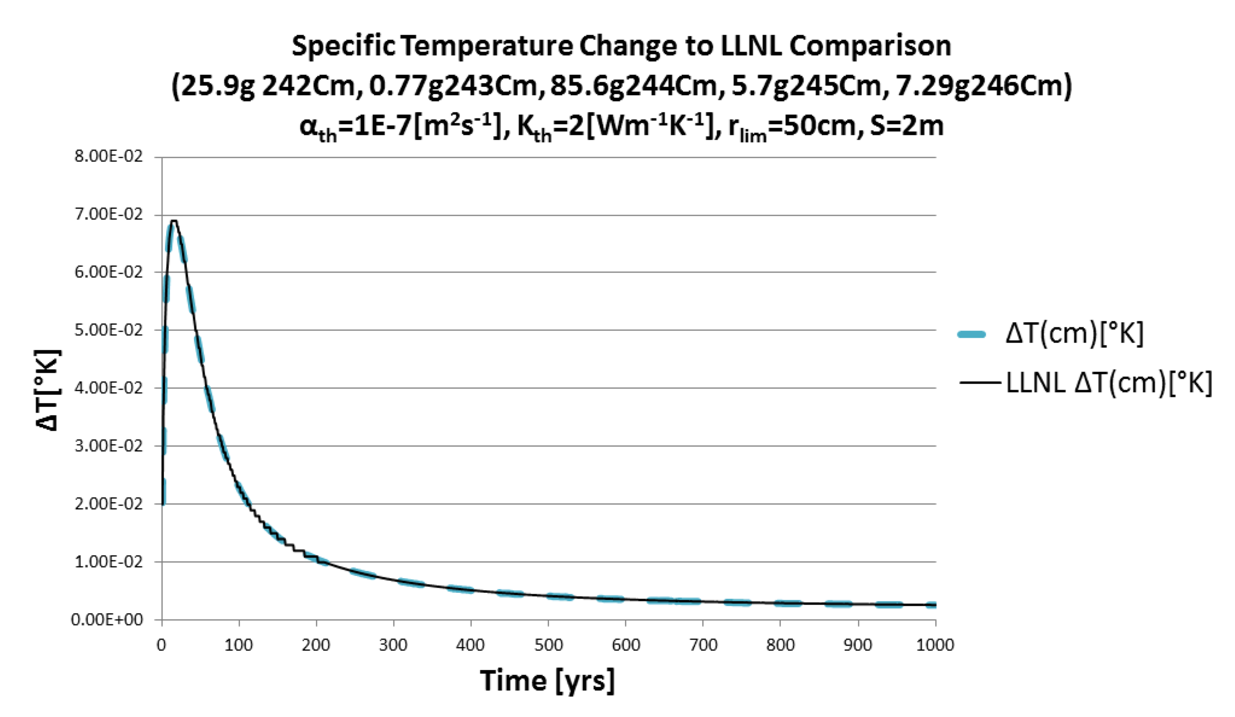
\includegraphics[width=\columnwidth]{./chapters/methodology/thermal_models/CmValidation.eps}
\end{center}
\caption{This comparison of \gls{STC} calculated thermal response from $Cm$ 
inventory per MTHM in 51GWd burnup UOX PWR fuel compares favorably with results 
from the semi-analytic model from LLNL.} 
\label{fig:CmValidation}
\end{figure}

\begin{figure}[htp!]
\begin{center}
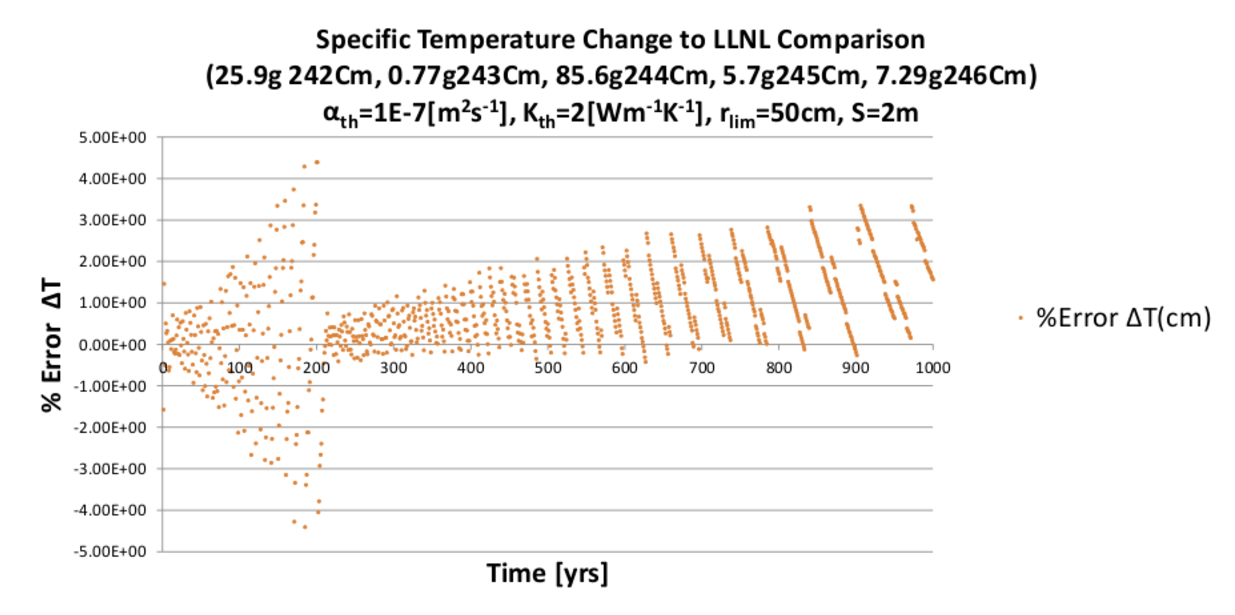
\includegraphics[width=\columnwidth]{./chapters/methodology/thermal_models/CmPercentError.eps}
\end{center}
\caption{Percent error between the semi-analytic model from LLNL and the \gls{STC} 
calculated thermal response from $Cm$ inventory per MTHM in 51GWd burnup UOX 
PWR fuel demonstrates a maximum percent error of 4.4\%.}
\label{fig:CmPercentError}
\end{figure}
% Unit Test Results
In addition to this validation effort, continual verification of code behavior 
is enabled by a suite of unit tests packaged with the tool. These tests are 
provided along with the source code so that they may be performed to evaluate 
the implementated behavior of units of functionality within the interpolation 
and specific temperature change algorithms even as the code is improved in the 
future.  

% \include{chaps/conclusions}

%% etc, etc.

%% Do you have appendices?  If so, add them here, just like chapters.
% \begin{appendices}
% \include{backmatter/appendix1}
% \end{appendices}

%% Are you a big nerd with a colophon?  Add it here.
\begin{colophon}

This template uses Gyre Pagella by default.  (I used Arno Pro in my dissertation.)

Feel free to give me a shout-out in your colophon or acks if this template is useful for you.  Good luck!

\end{colophon}

%% McBride is a very nice style (some version is included in this distribution)
\bibliographystyle{mcbride}
\bibliography{prelim}

%% Want an index?  Neither did I.
%\printindex

\end{document}
